% Created by tikzDevice version 0.10.1 on 2017-12-04 16:18:56
% !TEX encoding = UTF-8 Unicode
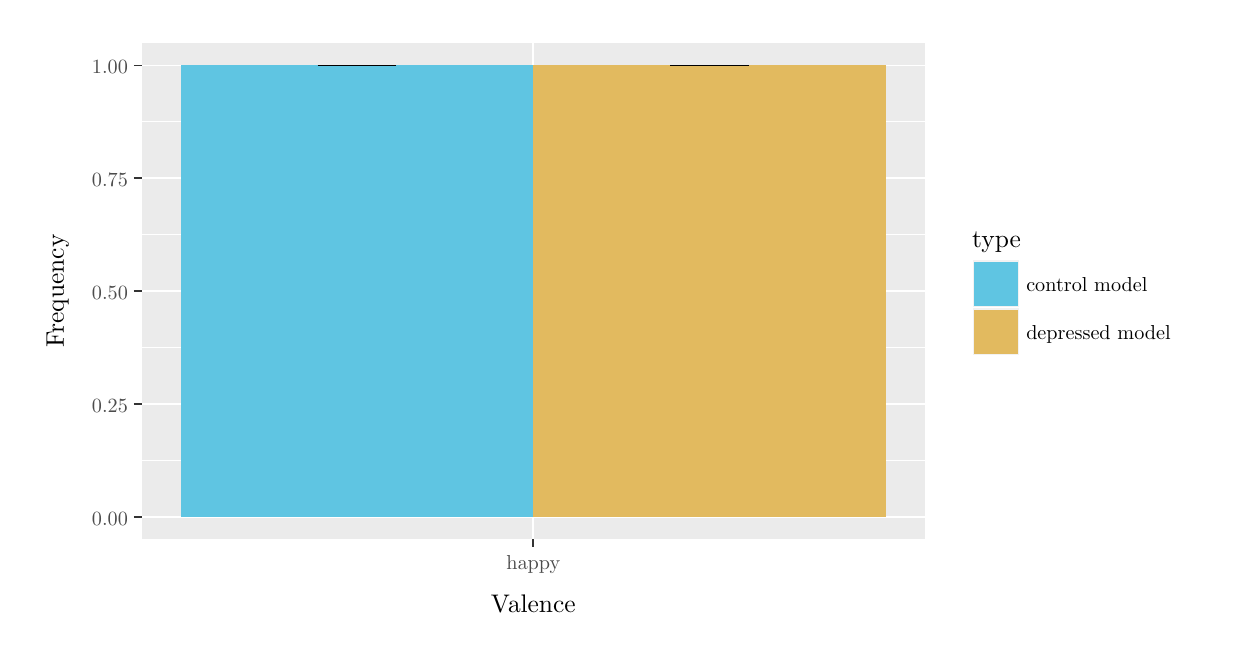
\begin{tikzpicture}[x=1pt,y=1pt]
\definecolor{fillColor}{RGB}{255,255,255}
\path[use as bounding box,fill=fillColor,fill opacity=0.00] (0,0) rectangle (433.62,216.81);
\begin{scope}
\path[clip] (  0.00,  0.00) rectangle (433.62,216.81);
\definecolor{drawColor}{RGB}{255,255,255}
\definecolor{fillColor}{RGB}{255,255,255}

\path[draw=drawColor,line width= 0.6pt,line join=round,line cap=round,fill=fillColor] (  0.00,  0.00) rectangle (433.62,216.81);
\end{scope}
\begin{scope}
\path[clip] ( 41.17, 31.92) rectangle (324.25,211.31);
\definecolor{fillColor}{gray}{0.92}

\path[fill=fillColor] ( 41.17, 31.92) rectangle (324.25,211.31);
\definecolor{drawColor}{RGB}{255,255,255}

\path[draw=drawColor,line width= 0.3pt,line join=round] ( 41.17, 60.46) --
	(324.25, 60.46);

\path[draw=drawColor,line width= 0.3pt,line join=round] ( 41.17,101.23) --
	(324.25,101.23);

\path[draw=drawColor,line width= 0.3pt,line join=round] ( 41.17,142.00) --
	(324.25,142.00);

\path[draw=drawColor,line width= 0.3pt,line join=round] ( 41.17,182.77) --
	(324.25,182.77);

\path[draw=drawColor,line width= 0.6pt,line join=round] ( 41.17, 40.07) --
	(324.25, 40.07);

\path[draw=drawColor,line width= 0.6pt,line join=round] ( 41.17, 80.84) --
	(324.25, 80.84);

\path[draw=drawColor,line width= 0.6pt,line join=round] ( 41.17,121.61) --
	(324.25,121.61);

\path[draw=drawColor,line width= 0.6pt,line join=round] ( 41.17,162.39) --
	(324.25,162.39);

\path[draw=drawColor,line width= 0.6pt,line join=round] ( 41.17,203.16) --
	(324.25,203.16);

\path[draw=drawColor,line width= 0.6pt,line join=round] (182.71, 31.92) --
	(182.71,211.31);
\definecolor{fillColor}{RGB}{226,186,95}

\path[fill=fillColor] (182.71, 40.07) rectangle (310.10,203.16);
\definecolor{fillColor}{RGB}{95,197,226}

\path[fill=fillColor] ( 55.33, 40.07) rectangle (182.71,203.16);
\definecolor{drawColor}{RGB}{0,0,0}

\path[draw=drawColor,line width= 0.6pt,line join=round] (232.25,203.16) --
	(260.56,203.16);

\path[draw=drawColor,line width= 0.6pt,line join=round] (246.41,203.16) --
	(246.41,203.16);

\path[draw=drawColor,line width= 0.6pt,line join=round] (232.25,203.16) --
	(260.56,203.16);

\path[draw=drawColor,line width= 0.6pt,line join=round] (104.87,203.16) --
	(133.17,203.16);

\path[draw=drawColor,line width= 0.6pt,line join=round] (119.02,203.16) --
	(119.02,203.16);

\path[draw=drawColor,line width= 0.6pt,line join=round] (104.87,203.16) --
	(133.17,203.16);
\end{scope}
\begin{scope}
\path[clip] (  0.00,  0.00) rectangle (433.62,216.81);
\definecolor{drawColor}{gray}{0.30}

\node[text=drawColor,anchor=base east,inner sep=0pt, outer sep=0pt, scale=  0.73] at ( 36.22, 37.04) {0.00};

\node[text=drawColor,anchor=base east,inner sep=0pt, outer sep=0pt, scale=  0.73] at ( 36.22, 77.81) {0.25};

\node[text=drawColor,anchor=base east,inner sep=0pt, outer sep=0pt, scale=  0.73] at ( 36.22,118.58) {0.50};

\node[text=drawColor,anchor=base east,inner sep=0pt, outer sep=0pt, scale=  0.73] at ( 36.22,159.36) {0.75};

\node[text=drawColor,anchor=base east,inner sep=0pt, outer sep=0pt, scale=  0.73] at ( 36.22,200.13) {1.00};
\end{scope}
\begin{scope}
\path[clip] (  0.00,  0.00) rectangle (433.62,216.81);
\definecolor{drawColor}{gray}{0.20}

\path[draw=drawColor,line width= 0.6pt,line join=round] ( 38.42, 40.07) --
	( 41.17, 40.07);

\path[draw=drawColor,line width= 0.6pt,line join=round] ( 38.42, 80.84) --
	( 41.17, 80.84);

\path[draw=drawColor,line width= 0.6pt,line join=round] ( 38.42,121.61) --
	( 41.17,121.61);

\path[draw=drawColor,line width= 0.6pt,line join=round] ( 38.42,162.39) --
	( 41.17,162.39);

\path[draw=drawColor,line width= 0.6pt,line join=round] ( 38.42,203.16) --
	( 41.17,203.16);
\end{scope}
\begin{scope}
\path[clip] (  0.00,  0.00) rectangle (433.62,216.81);
\definecolor{drawColor}{gray}{0.20}

\path[draw=drawColor,line width= 0.6pt,line join=round] (182.71, 29.17) --
	(182.71, 31.92);
\end{scope}
\begin{scope}
\path[clip] (  0.00,  0.00) rectangle (433.62,216.81);
\definecolor{drawColor}{gray}{0.30}

\node[text=drawColor,anchor=base,inner sep=0pt, outer sep=0pt, scale=  0.73] at (182.71, 20.91) {happy};
\end{scope}
\begin{scope}
\path[clip] (  0.00,  0.00) rectangle (433.62,216.81);
\definecolor{drawColor}{RGB}{0,0,0}

\node[text=drawColor,anchor=base,inner sep=0pt, outer sep=0pt, scale=  0.92] at (182.71,  5.50) {Valence};
\end{scope}
\begin{scope}
\path[clip] (  0.00,  0.00) rectangle (433.62,216.81);
\definecolor{drawColor}{RGB}{0,0,0}

\node[text=drawColor,rotate= 90.00,anchor=base,inner sep=0pt, outer sep=0pt, scale=  0.92] at ( 13.08,121.61) {Frequency};
\end{scope}
\begin{scope}
\path[clip] (  0.00,  0.00) rectangle (433.62,216.81);
\definecolor{fillColor}{RGB}{255,255,255}

\path[fill=fillColor] (335.63, 92.62) rectangle (428.12,150.61);
\end{scope}
\begin{scope}
\path[clip] (  0.00,  0.00) rectangle (433.62,216.81);
\definecolor{drawColor}{RGB}{0,0,0}

\node[text=drawColor,anchor=base west,inner sep=0pt, outer sep=0pt, scale=  0.92] at (341.32,137.34) {type};
\end{scope}
\begin{scope}
\path[clip] (  0.00,  0.00) rectangle (433.62,216.81);
\definecolor{drawColor}{RGB}{255,255,255}
\definecolor{fillColor}{gray}{0.95}

\path[draw=drawColor,line width= 0.6pt,line join=round,line cap=round,fill=fillColor] (341.32,115.66) rectangle (358.67,133.00);
\end{scope}
\begin{scope}
\path[clip] (  0.00,  0.00) rectangle (433.62,216.81);
\definecolor{fillColor}{RGB}{95,197,226}

\path[fill=fillColor] (342.04,116.37) rectangle (357.96,132.29);
\end{scope}
\begin{scope}
\path[clip] (  0.00,  0.00) rectangle (433.62,216.81);
\definecolor{drawColor}{RGB}{255,255,255}
\definecolor{fillColor}{gray}{0.95}

\path[draw=drawColor,line width= 0.6pt,line join=round,line cap=round,fill=fillColor] (341.32, 98.31) rectangle (358.67,115.66);
\end{scope}
\begin{scope}
\path[clip] (  0.00,  0.00) rectangle (433.62,216.81);
\definecolor{fillColor}{RGB}{226,186,95}

\path[fill=fillColor] (342.04, 99.03) rectangle (357.96,114.95);
\end{scope}
\begin{scope}
\path[clip] (  0.00,  0.00) rectangle (433.62,216.81);
\definecolor{drawColor}{RGB}{0,0,0}

\node[text=drawColor,anchor=base west,inner sep=0pt, outer sep=0pt, scale=  0.73] at (360.84,121.30) {control model};
\end{scope}
\begin{scope}
\path[clip] (  0.00,  0.00) rectangle (433.62,216.81);
\definecolor{drawColor}{RGB}{0,0,0}

\node[text=drawColor,anchor=base west,inner sep=0pt, outer sep=0pt, scale=  0.73] at (360.84,103.96) {depressed model};
\end{scope}
\end{tikzpicture}
